\documentclass[]{auvsi_doc}
\setkeys{auvsi_doc.cls}{
	AUVSITitle={Fall 2018 Timeline},
	AUVSILogoPath={figs/logo.pdf}
}

\usepackage{tikz}
\usepackage{gantt}
%\usepackage{rotating}
\usepackage{pdflscape}
\usepackage{longtable}

\begin{document}
\section*{Fall 2018 Gantt Chart}
%\begin{sidewaysfigure}
%\begin{landscape}
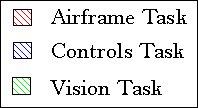
\includegraphics[]{figs/key.pdf}
\begin{center}
	% drawledgerline=true
\begin{gantt}[xunitlength=2.2cm]{24}{6}
	\begin{ganttitle}
		\titleelement{\textit{11/5}}{1}
		\titleelement{\textit{11/12}}{1}
		\titleelement{\textit{11/19}}{1}
		\titleelement{\textit{11/26}}{1}
		\titleelement{\textit{12/3}}{1}
		\titleelement{\textit{12/10}}{1}
	\end{ganttitle}
	\ganttbar[color=red]{\textbf{A1}}{0}{1}
	\ganttbarcon[color=red]{\textbf{A2}}{1}{1}
	\ganttbarcon[color=red]{\textbf{A3}}{2}{1}
	\ganttbar[color=red]{\textbf{A4}}{0}{1}
	\ganttbarcon[color=red]{\textbf{A5}}{1}{1}
	\ganttcon{2}{5}{2}{9}
	\ganttbar[color=blue]{\textbf{C1}}{0}{1}
	\ganttbarcon[color=blue]{\textbf{C2}}{1}{0.5}
	\ganttmilestonecon{\textbf{C3}}{2}
	\ganttbarcon[color=blue]{\textbf{C4}}{2}{0.5}
	\ganttmilestonecon{\textbf{C5}}{3}
	\ganttbarcon[color=green]{\textbf{V1}}{4}{1}
	\ganttbarcon{\textbf{MC1}}{5}{0.5}
	\ganttmilestonecon{\textbf{MC}}{6}
\end{gantt}
\end{center}
\newpage
\begin{center}
	\bgroup
	\def\arraystretch{1.25}%  1 is the default, change whatever you need
	\begin{longtable}{P{2cm}P{13cm}}
		\hline
		\textbf{Task ID} 	& \textbf{Description} \\
		\hline
		\textbf{A1} & Obtain new airframe \\
		\textbf{A2} & Assemble new airframe with RC components \\
		\textbf{A3} & Fly new airframe RC \\
		\textbf{A4} & Get last year's payload drop mechanism working \\
		\textbf{A5} & Pack all components into last year's plane (camera, payload, etc) \\
		\textbf{C1} & Carry out full missions with the plane and interop server in simulation  \\
		\textbf{C2} & Extensive testing and verification of subsystems for autonomous flight \\
		\textbf{C3} & Fly last year's plane in hardware autonomously without a payload \\
		\textbf{C4} & Extensive testing and verification of subsystems for autonomous flight and payload drop \\
		\textbf{C5} & Fly last year's plane in hardware autonomously with a payload \\
		\textbf{V1} & Capture images of targets in hardware \\
		\textbf{MC1} & Prepare for mock competition (simulation runs, setup, etc) \\
		\textbf{MC} & MOCK COMPETITION \\
		\hline
	\end{longtable}
	\egroup
\end{center}
%\end{landscape}
%\end{sidewaysfigure}

\end{document}